\section{系统设计}
\label{sec:design}

本小节将介绍系统设计。首先,简单地回顾系统整体架构。随后介绍算法核心中的模块设计与调用关系。接着,介绍算法核心中的数据结构与规划算法。最后,简要介绍服务器端与前端的模块结构关系与大概设计。

\begin{figure}[t]
  \centering
  
\includegraphics[width=\textwidth]{figures/system_arch}
  \caption{系统架构}
  \label{fig:system-arch}
\end{figure}

\subsection{系统架构}

如图 \ref{fig:system-arch} 中所示,系统由三大部分组成。(a) GUI负责信息展示、旅程展示、用户交互等。与服务器通信;(b) 服务器负责与GUI通信。管理已有的旅程信息。并且调用算法核心进行旅程规划;(c) 算法核心能够加载、管理城市线路信息,进行旅行规划,生成旅途信息等等。

\textsc{TravelAgency}系统的核心逻辑功能,都在算法核心中实现,包括:定义了城市线路信息的数据结构(图),从文件中加载读取城市、线路信息;定义了描述旅程的数据机构(可持久化链表),规划并生成旅程信息。注意当前旅程信息的保管不由算法核心完成,而由服务器完成,服务器将所有规划模拟的旅行保存在一个列表中,能够通过Websocket提供给前端用户界面。

程序当前的状态,包括当前时间,进行中的旅行等,都由前端GUI界面与服务器管理。当前时间保存在前端界面的逻辑中,前端界面根据旅程信息与当前时间实时渲染出旅行的状态。而当前的旅行列表,如前所述,保存在服务器中。并且能与前端实时通信,进行更新。

\subsection{算法核心中的数据结构}

本小节将介绍算法核心实现和使用的数据结构。

\subsubsection{城市}

城市是一个数据字典,如下所示。

\begin{lstlisting}[caption={城市数据结构}]
struct City
{
  int id; // 城市编号。是唯一标识符。
  int level; // 城市风险等级。2: 高风险; 1: 中风险; 0: 低风险。
  string name; // 城市名称。
}
\end{lstlisting}

\subsubsection{线路}

线路同样是一个数据字典,如下所示。

\begin{lstlisting}[caption={线路数据结构}]
struct Line
{
  int id; // 线路编号。是唯一标识符。
  LineType type; // 线路类型。enum LineType \{ Air, Subway, Highway \}
  int dep_time; // 出发时间。
  int duration; // 时长。
}
\end{lstlisting}

具体地,有$\text{duration} \in \mathds N_+, \text{dep\_time} \in \{ 0, 1, \cdots, 23 \}$。

\subsubsection{城市线路图}

城市线路图是一张图。并且通过\textbf{邻接表}来存储边的信息。具体如下所示。

\begin{lstlisting}[caption={线路数据结构}]
struct CityMap
{
  City cities[N];
  LinkedList<Line> lines[N];
}
\end{lstlisting}

其中,$N$为城市个数。\textit{注意上面的只是伪代码},真正的实现中使用了面向对象的设计,并且使用了 \lstinline{vector} 这样的STL类。\lstinline{LinkedList} 为我实现的链表。其实现如下所示。

\begin{lstlisting}[caption={链表数据结构}]
typedef struct LinkedNode<T> * LinkedList<T>;

struct LinkedNode<T>
{
  T val;
  LinkedNode<T> *next;
}
\end{lstlisting}

\begin{figure}[h]
  \centering
  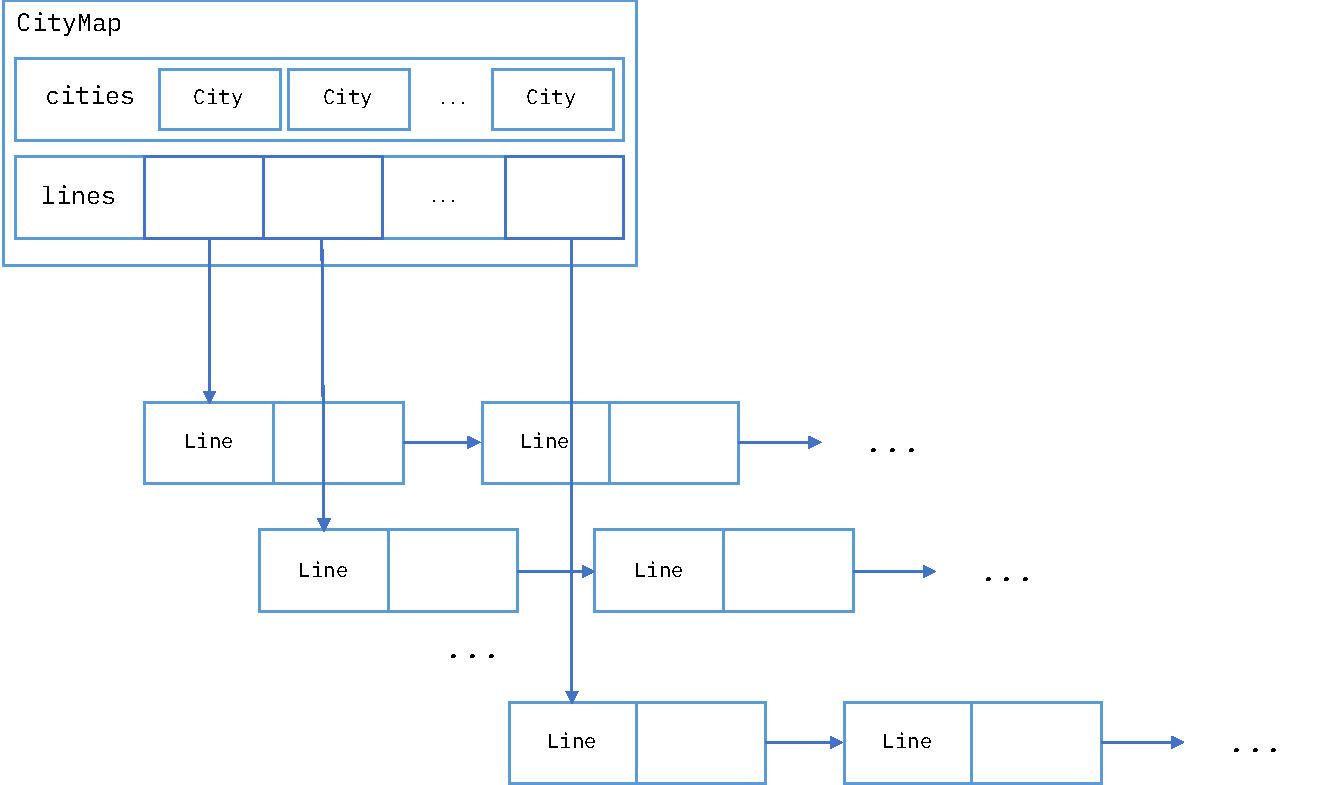
\includegraphics[width=0.7\textwidth]{figures/city_map_structure}
  \caption{城市线路图数据结构示意图}
  \label{fig:city-map-structure}
\end{figure}

实现中使用了C++的Template特性来使其能够适应不同的元素类型。

具体地,邻接表是一种利用链表存储图结构的数据结构,具有很好的空间复杂度。形式化地,
\begin{definition}[邻接表]
  对于一张图$\mathcal G = (\mathcal V, \mathcal E)$。利用一个映射$\varphi : \mathcal V \rightarrow \text{LinkedList<} \mathcal E \text{>}$来表示图的结构。具体地,$\varphi = c \mapsto \text{LinkedList} \{ l \in \mathcal E | c_s(l) = c \} $。也即为每一个节点映射一个存储边信息的链表,每一链表中包含对应节点出发的所有边。在实践中,映射往往由连续数组实现。
\end{definition}

对使用了邻接表存储的图而言,空间复杂度约为$\mathcal O(| \mathcal E |)$,对于一般的稀疏图而言,远远低于使用邻接矩阵存储的$\mathcal O(| \mathcal V |^2)$。

图 \ref{fig:city-map-structure} 中直观展示了城市线路图数据结构的主体结构。可以看到,数据结构中首先以数组存储了所有城市节点的信息。随后,以数组存储每一个城市的邻接表。每个城市的邻接表中保存了从该城市出发的所有线路信息。

\subsubsection{旅行方案}

旅行方案的本质是记录需要搭乘的线路。除此以外,还需要记录如出发地、目的地、总时长、风险值等辅助信息,方便接下来的处理。考虑到规划算法乃至于整套系统运行过程中,旅行方案有一个非常重要的特征:\textbf{在规划、生成旅行方案,乃至于接下来处理、展示方案的过程中,只涉及方案的生成、步骤的增添、路线的增长,不涉及对旅行方案中已有步骤的修改。}而另一个事实是,\textbf{在运行规划算法的过程中,会产生许多的临时、中间方案,而很多方案是从同一个中间方案延伸出来的,这些方案的路线中包含共享的部分。}

\paragraph{可持久化链表} 基于上面的特征和事实,我利用了\emph{可持久化链表 (persistent linked list)}来描述旅行方案。可持久化链表为可持久化数据结构中的一种,是\emph{无法原地修改 (immutable)}的数据结构。无法在原地修改的含义为,在修改时总是产生一个新的副本,而非在原来的链表上进行修改。这意味着无论在任何时候,先前产生的链表都不会因为后面产生的修改而被意外的改动。

可持久化链表在增加节点时非常简单。由于可持久化的性质保证了之前的链表不可能被修改,因而共享了元素的链表可以直接共用相同的部分。这带来了时间与空间上的优势。

\begin{figure}[t]
	\centering
	\subfloat[修改前]{
		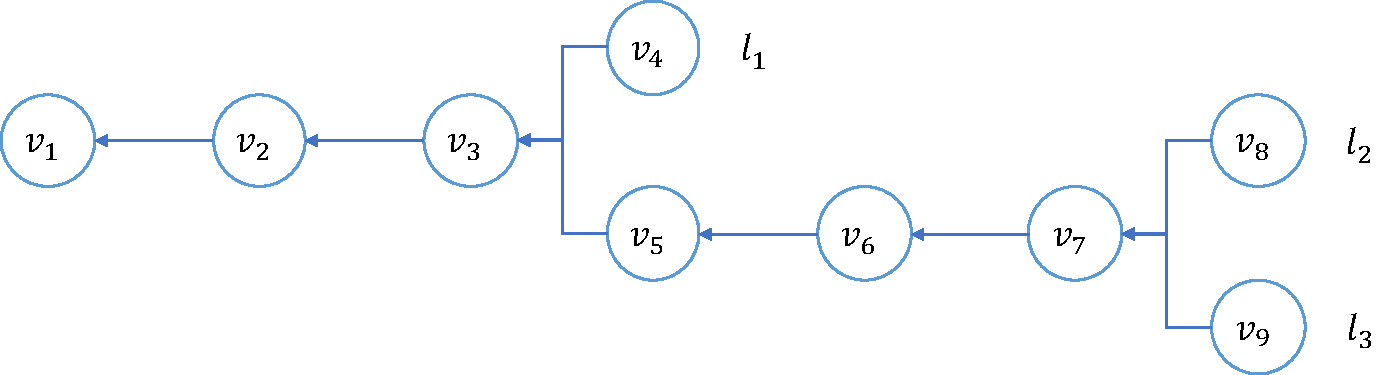
\includegraphics[width=0.5\textwidth]{figures/pll_example}
		\label{fig:pll-example-before}
	}
	\subfloat[修改后]{
		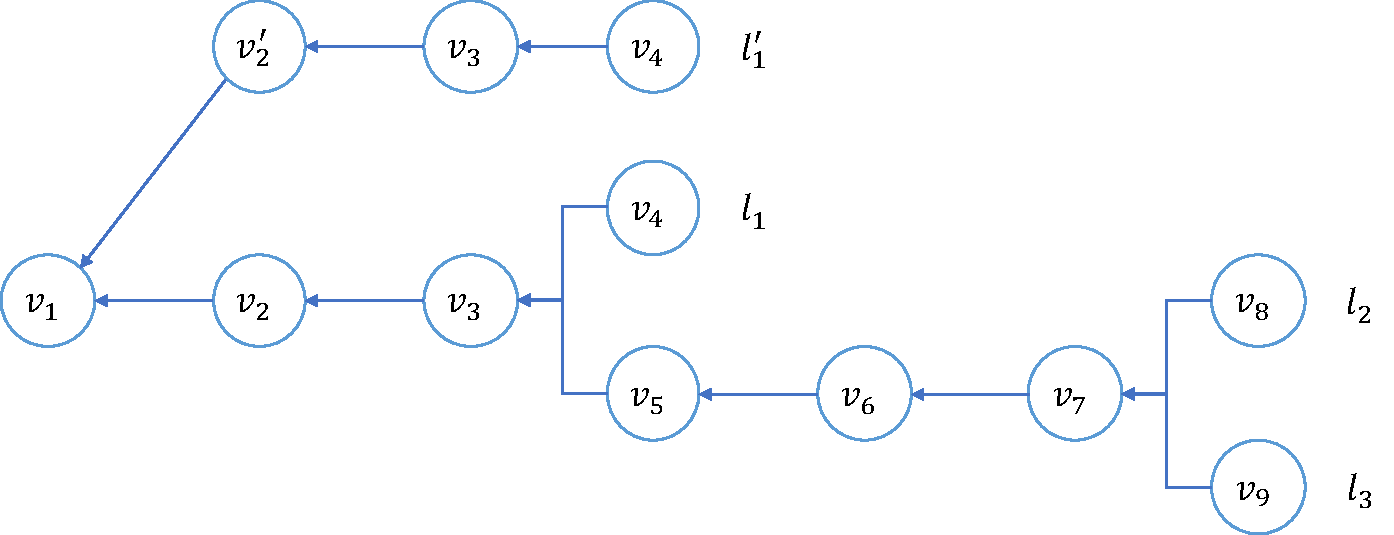
\includegraphics[width=0.5\linewidth]{figures/pll_example_mod}
		\label{fig:pll-example-mod}
	}
	\caption{可持久化链表的修改}
	\label{fig:pll-example}
\end{figure}

然而,在需要对链表的某一中间节点进行修改时将产生大量的复制。图 \ref{fig:pll-example-before} 中是采用了可持久化结构的三个链表。如果要将链表$l_1$从$v_4 \rightarrow v_3 \rightarrow v_2 \rightarrow v_1$修改为$v_4 \rightarrow v_3 \rightarrow v_2^\prime \rightarrow v_1$也即图 \ref{fig:pll-example-mod} 中的$l_1^\prime$,则需要将除了$v_1, v_2$之外的部分都进行复制。原因是在可持久化链表中,不能对之前的某个节点进行修改。

\paragraph{用可持久化链表描述旅行方案}

然而,在\textsc{TravelAgency}中,用可持久化链表来描述旅行方案可以规避上面提到的弱点:在规划的过程中,并不涉及对之前节点的修改,只涉及链表的延伸。因而在此应用场景中,可持久化链表能够实现高效的内存共享,快速的链表延伸,非常适合用于描述旅行方案。

具体地,旅行方案的数据结构可以如下表达。

\begin{lstlisting}[caption={旅行方案数据结构}]
struct Journey
{
  const int src; // 出发城市编号。
  const int dest; // 目的城市编号。
  const int dep_time; // 出发时间。
  const int arrive_time; // 到达时间。
  const int line; // 乘坐线路。
  const int length; // 总时长。
  const double risk; // 风险。
  const Journey *prev; // 上一段旅途方案。
}
\end{lstlisting}

\begin{algorithm}[t]
\caption{\textsc{Concat}($j$, $l$): $\mathcal J \times \mathcal E \rightarrow \mathcal J$}
\label{algo:concat-journey}
\KwIn{$j \in \mathcal J$:上一段的旅程方案;$l \in \mathcal E$:下一步搭乘的线路}
\KwOut{$j^\prime$:新的旅程方案}
\textsc{Assert}($j.dest = c_s(l)$)\;
$j^\prime.src \gets j.src$\;
$j^\prime.dest \gets c_d(l)$\;
$j^\prime.dep\_time \gets  j.dep\_time$\;
$j^\prime.arrive\_time \gets t_d(l) \oplus \tau(d)$\tcp*{$\oplus$ is mod-24 addition}
$j^\prime.line \gets l$\;
$j^\prime.length \gets j.length + \| t_d(l) - j.arrive\_time \| + \tau(l)$\;
$j^\prime.risk \gets j.risk + r_c(j.dest)\| t_d(l) - j.arrive\_time \| + r_l(l) r_c(j.dest) \tau(l)$\;
$j^\prime.prev \gets j$\;
\Return $j^\prime$\;
\end{algorithm}

而延伸旅行方案的算法如算法 \ref{algo:concat-journey} 中所示。其中$\mathcal J$为旅行方案的集合。注意到在数据结构定义中,所有的域都是不可修改的。算法中的赋值类似于初始化的过程,一旦完成赋值,离开算法,旅行方案中的域都无法修改。

\paragraph{可持久化链表的实现}

在实际的实现中,利用了C++中提供的 \lstinline{shared_ptr}。其最大的优势在于,能够方便、高效、不易出错地管理对同一片内存空间的引用。对算法运行过程中,产生的旅行方案的任一部分,只要当前的作用域内还包含对其的直接或间接引用,它就会被保留。当不再有对某一部分的任何引用时(如因发现更优解而将原先的解丢弃),将直接释放其内存。既不会产生内存泄漏,也不会对某一片内存产生多次或提前释放,产生不可预知的错误。

\subsection{算法核心中两种策略的规划算法}

\subsubsection{最小风险旅行规划算法}

\textsc{TravelAgency}系统中,最小风险规划算法的设计基于\emph{SPFA (shortest path faster algorithm)},也即带有队列优化的\emph{Bellman-ford}算法。是非常常用、高效的图上单源最短路算法。

然而,为了进行最小风险规划,系统并不直接在城市图上运行SPFA算法,而是在时间-城市图上。时间-城市图从城市图生成,其中的每一个节点都是包含了当前城市和当前时间的偶对。

\begin{wrapfigure}{r}{0.57\textwidth}
\begin{minipage}{0.57\textwidth}
\begin{algorithm}[H]
\caption{\textsc{ConstructTemporalEdges}($\mathcal G$)}
\label{algo:construct-temporal-edges}
\KwIn{$\mathcal G$: 输入城市图}
\KwOut{$\mathcal E^\prime$:时间-城市图的边集}
$\mathcal E^\prime \gets \emptyset$\;
\For{$e \in \mathcal E$}{
  $t_a \gets t_d(e) \oplus \tau(e)$\;
  $c_1 \gets c_s(e)$\;
  $c_2 \gets c_d(e)$\;
  \For{$t \in \mathds H$}{
    $\mathcal E^\prime \gets \mathcal E^\prime \cup \{ \langle (c_1, t), (c_2, t_a) \rangle \}$\;
  }
}
\Return $\mathcal E^\prime$\;
\end{algorithm}
\end{minipage}
\end{wrapfigure}

\begin{definition}[时间-城市图]
  对于一张城市图$\mathcal G = (\mathcal V, \mathcal E, r_c, r_l, t_d, t_a, \tau, v_s, v_d)$,其对应的时间-城市图为$\mathcal G^\prime = (\mathcal V^\prime, \mathcal E^\prime)$。其中$\mathcal V^\prime =  \mathcal V \times \mathds H$。其中$\mathds H \triangleq \{ 0, 1, \cdots, 23 \}$为一天中可能的时刻集合。集合$\mathcal E^\prime$的生成由算法 \ref{algo:construct-temporal-edges} 描述。注意,$t \oplus \tau \triangleq (t + \tau) \% 24$为模24加法。在模24加法下可以计算出线路的抵达时刻。
\end{definition}

\begin{figure}[t]
  \centering
  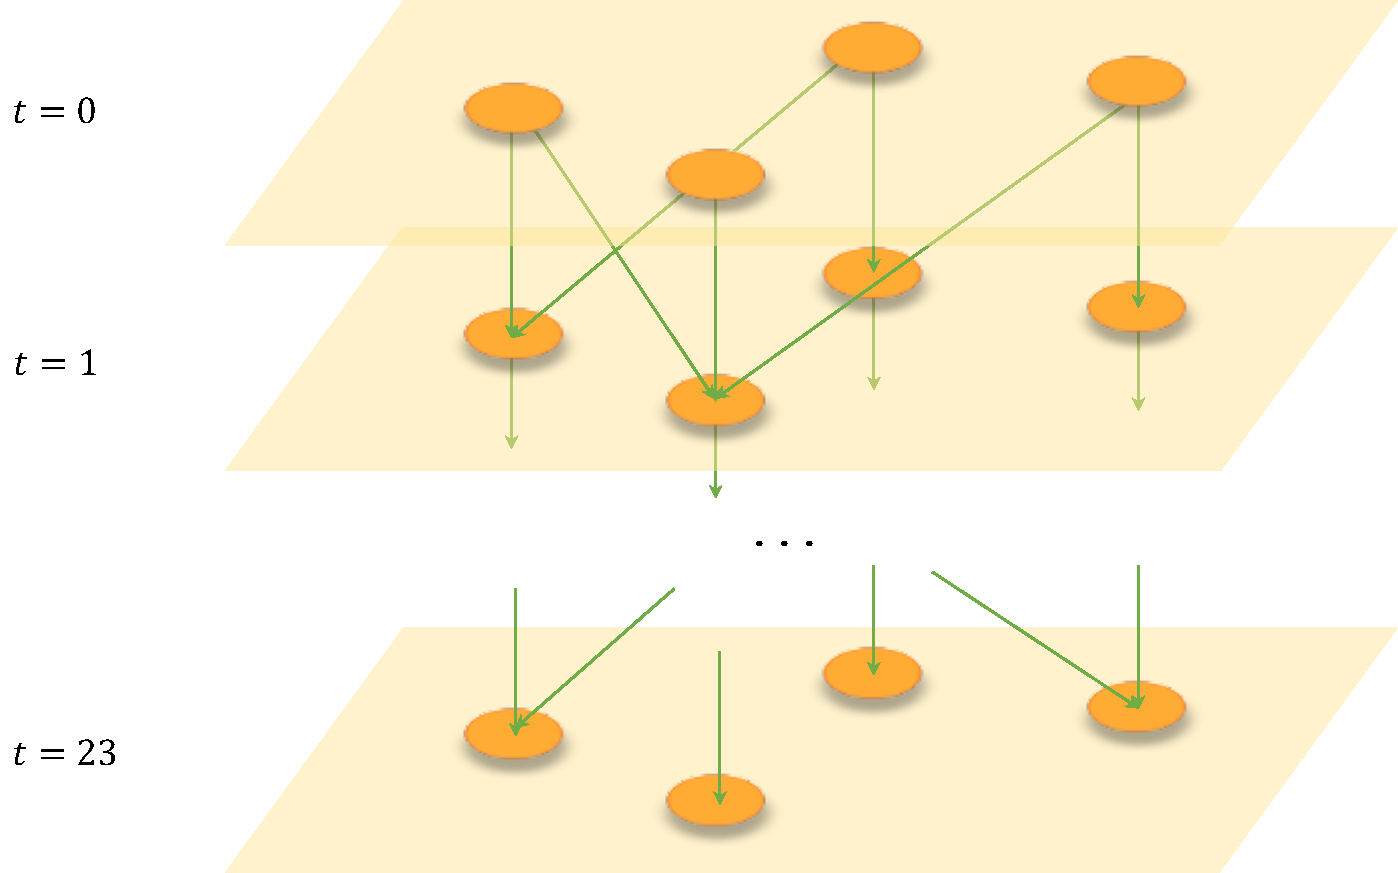
\includegraphics[width=0.7\textwidth]{figures/time_map}
  \caption{时间-城市图}
  \label{fig:time-map}
\end{figure}

图 \ref{fig:time-map} 中是一张时间-城市图的例子。其中的每一层都代表了一个时刻。图中的每个节点不仅包含城市信息,也有对应的时刻。图中的边不止是在城市之间转移,也在不同的时刻之间转移。使用时间-城市图,而非简单的城市图,能够更加准确、全面地描述出旅行中的状态信息。当某一旅客处于节点$(c, t)$时,则代表他当前处于城市$c$,当前时刻为$t$。在获知了当前时间$t$和当前地点$c$之后,旅客乘坐从当地出发的各条线路需要的等待时间、等待风险等,便可以明确地计算出来,乃至于从状态$(c, t)$到其他状态的最小风险路径,也可以通过算法方便地求解出来。

\begin{algorithm}[t]
\caption{\textsc{MinRiskSolver}($\mathcal G, c_1, c_2, t_0$)}
\label{algo:min-risk-solver}
\KwIn{$\mathcal G$:输入城市图;$c_1, c_2$:出发城市、目的城市;$t_0$:出发时间}
\KwOut{$j$:旅行方案}
$\bm J \in \mathcal J^{ |\mathcal V| \times |\mathcal H| }$\;
$\bm J[c_1, t_0] \gets $\textsc{Initial}($c_1, t_0$)\;
$q \gets $\textsc{Queue}$[ ]$\;
\textsc{Push}($q, \langle c_1, t_0 \rangle$)\;
\While{$q$ is not empty}{
  $\langle c, t \rangle \gets $\textsc{Pop}($q$)\;
  \For{$e \in \{ e_0 \in \mathcal E \mid c_s(e_0) = c \}$}{
    $j \gets $\textsc{Concat}$(\bm J[c, t], e)$\;
    $\langle c^\prime, t^\prime \rangle \gets \langle j.dest, j.arrive\_time \rangle$\;
    \If{$\langle c^\prime, t^\prime \rangle$ has not been reached $\vee \ j.risk < \bm J[c^\prime, t^\prime].risk$}{
      $\bm J [c^\prime, t^\prime] \gets j$\;
      \If{$\langle c^\prime, t^\prime \rangle \notin q$}{
        \textsc{Push}($q, \langle c^\prime, t^\prime \rangle$)\;
      }
    }
  }
  $j \gets $ empty\;
  \For{$t \in \mathds H$}{
    \If{$\bm J[c_2, t]$ is not empty}{
      \If{$j$ is empty $\vee$ $j.risk > \bm J[c_2, t].risk$}{
        $j \gets \bm J[c_2, t]$\;
      }
    }
  }
  
  \Return $j$\;
}
\end{algorithm}

求解最小风险策略旅行方案的算法如算法 \ref{algo:min-risk-solver} 中所示。算法并没有设计显示地构造时间-城市图的边集,因为这张图可以是一张\emph{隐含}图。在SPFA算法中要进行状态转移,更新状态最优解的时候,可以根据城市线路图中的边隐含地计算出时间-城市图中的边并进行处理。因而,时间-城市图中的边结构在算法运行的始末都不曾被显示地构造出来,这样将其视为隐含图的处理提高了算法的时间与空间效率。基于SPFA的算法 \ref{algo:min-risk-solver} 中使用了队列数据结构。其具有这些方法:\textsc{Queue}能够从一个列表构造出一个队列;\textsc{Push}($q, v$)将元素$v$放入队列$q$中;\textsc{Pop}($q$)从队列$q$中取出一个元素并返回。

算法 \ref{algo:min-risk-solver} 中使用的\textsc{Initial}方法,定义如算法 \ref{algo:initial} 中所示,作用是生成一个包含出发地点的初始化节点,供后续的算法处理。

\subsubsection{限时最小风险旅行规划算法}

\begin{wrapfigure}{r}{0.5\textwidth}
\begin{minipage}{0.5\textwidth}
\begin{algorithm}[H]
\caption{\textsc{Initial}($c_0$, $t_d$)}
\label{algo:initial}
\KwIn{$c_0$: 起始城市;$t_d$:出发时间}
\KwOut{$j$:供后续算法处理的起始旅行方案}
$j.src \gets c_0$\;
$j.dest \gets c_0$\;
$j.dep\_time \gets t_d$\;
$j.arrive\_time \gets t_d$\;
$j.line \gets $ null\;
$j.length \gets 0$\;
$j.risk \gets 0$\;
$j.prev \gets $ null\;
\Return $j$\;
\end{algorithm}
\end{minipage}
\end{wrapfigure}

限时最小风险策略的规划算法,同样能够基于SPFA实现。一个直觉的想法是在最小风险策略SPFA的状态更新过程中,直接丢弃超时的方案。这样可以保证能求出合法的解,然而却是错误的。下面给出一个反例。

\textbf{时间-城市图上带时间约束的SPFA算法的反例} \quad 考虑图 \ref{fig:bad-graph-example} 中的例子。若要求从$v_1$到$v_3$的限时最小风险路径,7点整出发,限制时间为30h,假设$v_1$到$v_2$有两种方案,一条时长为1h,风险为2;另一条时长为25h,风险为1。从$v_2$到$v_3$的最佳方案耗时6h,风险为2。通过肉眼观察可以发现,最佳路径时长为7h,风险为4。
\begin{figure}[t]
\centering
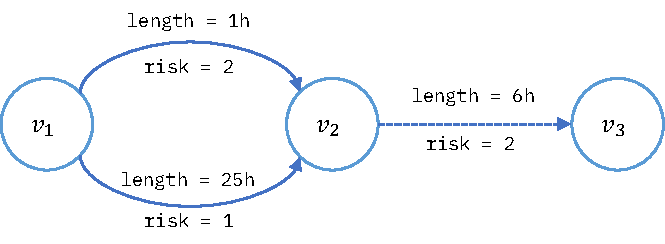
\includegraphics[width=0.7\textwidth]{figures/bad_graph_example}
\caption{例子}
\label{fig:bad-graph-example}
\end{figure}
然而在SPFA算法运行过程中,由于时长为1h的路径的风险大于另一条,时长为1h的路径会被丢弃,导致算法找不到可行解,错误地认为不可能在限制时间内到达目的地。

\textbf{时长-城市图} \quad 要解决上述问题的方法很简单,只需要将原本的时间-城市图,改为时长-城市图。也即图中的每一节点,从原先的包含当前时间与当前所在城市,改为当前从旅途开始已经过去的时间。对于某一城市图$\mathcal G$,限制时间为$\Gamma$,定义$\mathds D(\Gamma) \triangleq \{ 0, 1, 2, \cdots, \Gamma \}$,则时长-城市图的点集$\mathcal V^\prime = \mathcal V \times \mathds D(\Gamma)$,边集也可以像时间-城市图那样定义,并且无需显式构造。

限时最小风险的旅行规划算法与最小风险算法相类似。区别是节点定义的变化,以及在状态更新时需要考虑时长。具体定义如算法 \ref{algo:limited-time-min-risk-solver} 中所示。

\begin{algorithm}[t]
\caption{\textsc{LimitedTimeMinRiskSolver}($\mathcal G, c_1, c_2, t_0, \Gamma$)}
\label{algo:limited-time-min-risk-solver}
\KwIn{$\mathcal G$:输入城市图;$c_1, c_2$:出发城市、目的城市;$t_0$:出发时间;$\Gamma$:时间限制}
\KwOut{$j$:旅行方案}
$\bm J \in \mathcal J^{ |\mathcal V| \times |\Gamma + 1| }$\;
$\bm J[c_1, 0] \gets $\textsc{Initial}($c_1, t_0$)\;
$q \gets $\textsc{Queue}$[ ]$\;
\textsc{Push}($q, \langle c_1, 0 \rangle$)\;
\While{$q$ is not empty}{
  $\langle c, t \rangle \gets $\textsc{Pop}($q$)\;
  \For{$e \in \{ e_0 \in \mathcal E \mid c_s(e_0) = c \}$}{
    $j \gets $\textsc{Concat}$(\bm J[c, t], e)$\;
    $\langle c^\prime, t^\prime \rangle \gets \langle j.dest, j.length \rangle$\;
    \If{$j.length \leq \Gamma$ $\wedge$ $(\langle c^\prime, t^\prime \rangle$ has not been reached $\vee \ j.risk < \bm J[c^\prime, t^\prime].risk)$}{
      $\bm J [c^\prime, t^\prime] \gets j$\;
      \If{$\langle c^\prime, t^\prime \rangle \notin q$}{
        \textsc{Push}($q, \langle c^\prime, t^\prime \rangle$)\;
      }
    }
  }
  $j \gets $ empty\;
  \For{$t \in \mathds D(\Gamma)$}{
    \If{$\bm J[c_2, t]$ is not empty}{
      \If{$j$ is empty $\vee$ $j.risk > \bm J[c_2, t].risk$}{
        $j \gets \bm J[c_2, t]$\;
      }
    }
  }
  
  \Return $j$\;
}
\end{algorithm}

\subsubsection{算法性能分析}

最小风险与限时最小风险规划算法都基于SPFA。查阅资料可知SPFA在实验中的平均时间复杂度约为$\mathcal O(|\mathcal E^\prime|)$,最坏时间复杂度为$\mathcal O(|\mathcal V^\prime| |\mathcal E^\prime|)$其中$\mathcal V^\prime, \mathcal E^\prime$分别为隐含图的点集与边集。

因而,对于最小风险策略规划算法而言,可以认为算法的时间复杂度约为$\mathcal O(|\mathds H| |\mathcal E|) = \mathcal O(|\mathcal E|)$。对于限时最小风险规划算法而言,时间复杂度约为$\mathcal O(| \Gamma + 1 | | \mathcal E |)$。他们关于线路数量都是线性的。

\subsection{服务器的设计}

本小节将介绍服务器的功能与设计实现。首先介绍功能。
\begin{enumerate}[(a)]
  \item 存储规划好的旅程信息。服务器将保存算法核心规划好的旅程信息,存入旅程列表。并且在前端界面要求的时候发送给前端,由前端展现给用户。
  \item 与前端界面通信。服务器需要响应前端请求,返回相应数据。
  \item 调用算法核心中的算法。服务器通过加载动态库,来调用算法核心实现的算法,进行旅行方案的规划。
\end{enumerate}

\begin{figure}[t]
  \centering
  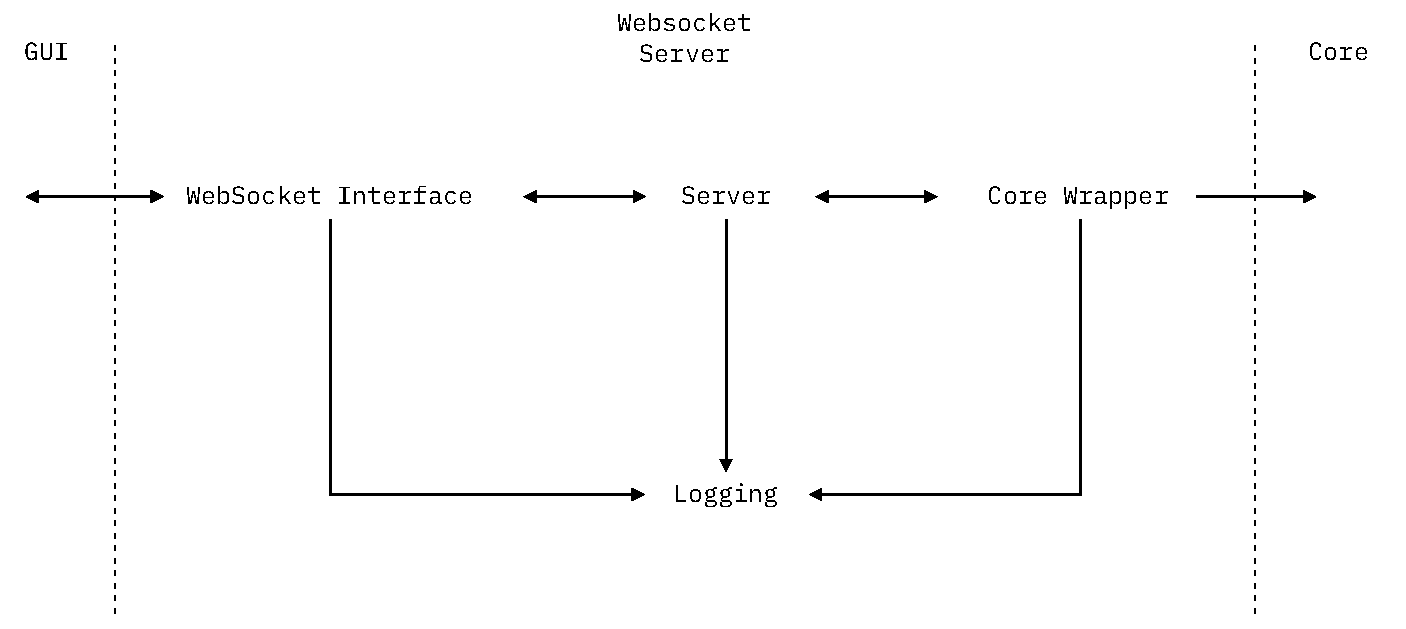
\includegraphics[width=0.7\textwidth]{figures/server_arch}
  \caption{服务器模块结构图}
  \label{fig:server-arch}
\end{figure}

{\setstretch{1.5}
服务器的模块结构图如图 \ref{fig:server-arch} 中所示。服务器主要有如下模块。
\begin{enumerate}[(a)]
  \item \textbf{WebSocket接口 (WebSocket Interface)}。该模块负责与前端进行通信。使用Python的 \lstinline{websockets} 与 \lstinline{asyncio} 库实现。考虑到接口的负载并不大,一般而言只有一个前端与之通信,因而 \lstinline{asyncio} 提供的并发实现完全足够。
  \item \textbf{服务器 (Server)}。服务器模块包含对前端请求的处理逻辑,以及包含了对服务器状态(动态库接口句柄,旅行方案列表等)的定义与管理。
  \item \textbf{日志记录 (Logging)}。由Python的 \lstinline{logging} 库实现。能够对日志信息进行分级记录与显示。
  \item \textbf{核心库封装 (Core Wrapper)}。核心库封装模块通过 \lstinline{ctypes} 调用C++编写的动态库,并且将其中的函数封装为Python函数,将C++中定义的数据结构映射到Python中,定义相应的类。
\end{enumerate}}

\subsection{前端用户界面的设计}

前端界面主要要实现如下功能:
\begin{enumerate}
  \item 接受用户输入,交互式地添加、查看旅行。
  \item 实时显示城市信息、旅行状态,显示旅行线路、展示旅客状态等。
  \item 与服务器进行通信,添加旅行方案,要求规划旅行方案,要求获取城市、道路信息等。
  \item 管理当前时间状态,暂停、继续当前时间的进行,根据当前时间计算出各个旅程所处的状态等。
\end{enumerate}

\begin{figure}[t]
  \centering
  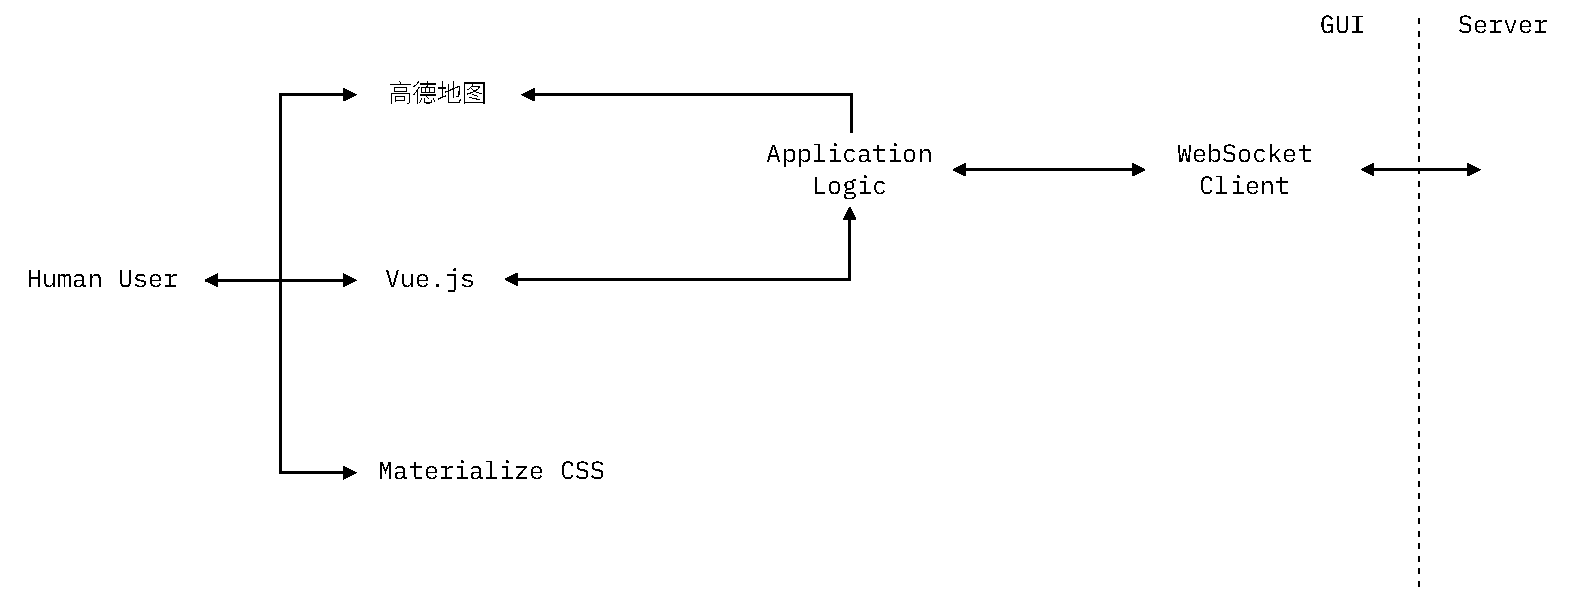
\includegraphics[width=0.7\textwidth]{figures/gui_arch}
  \caption{前端界面模块结构图}
  \label{fig:gui-arch}
\end{figure}

前端界面的模块结构如图 \ref{fig:gui-arch} 中所示。其功能分别如下:
\begin{enumerate}
  \item \textbf{高德地图、Vue.js、Materialize CSS}。这三个模块都负责前端界面的显示与交互。高德地图负责地图的显示、城市信息的绘制、旅程信息的绘制等等。Vue.js是非常常用的前端框架,负责右侧信息面板的交互事件管理与数据的渲染。并且也监听程序状态的变化,若有必要将根据变更的状态在高德地图中重新渲染。Materialize CSS也是常用的前端界面框架,能够提供Material Design风格的前端组件。
  \item \textbf{程序逻辑 (Application Logic)}。该模块实现了程序的主体逻辑。如如何响应用户事件、调用WebSocket客户端进行通信、如何响应WebSocket信息等等。并实现了地图的绘制逻辑。
  \item \textbf{WebSocket客户端 (WebSocket Client)}。该模块负责建立WebSocket连接,与服务器通信。
\end{enumerate}





















